\subsubsection{Spectrogram}
A spectrogram allows acquisition of data time-series. A spectrogram stores data with specified time intervals and can be displayed in a waterfall plot. It is also the function LuRaCs utilise for mobile measurements. If a GPS is connected, the geolocation data is automatically stored in the spectrogram. These measurements can be visualised on the embedded Map (or an online map).

\begin{figure}[H]
    \centering
    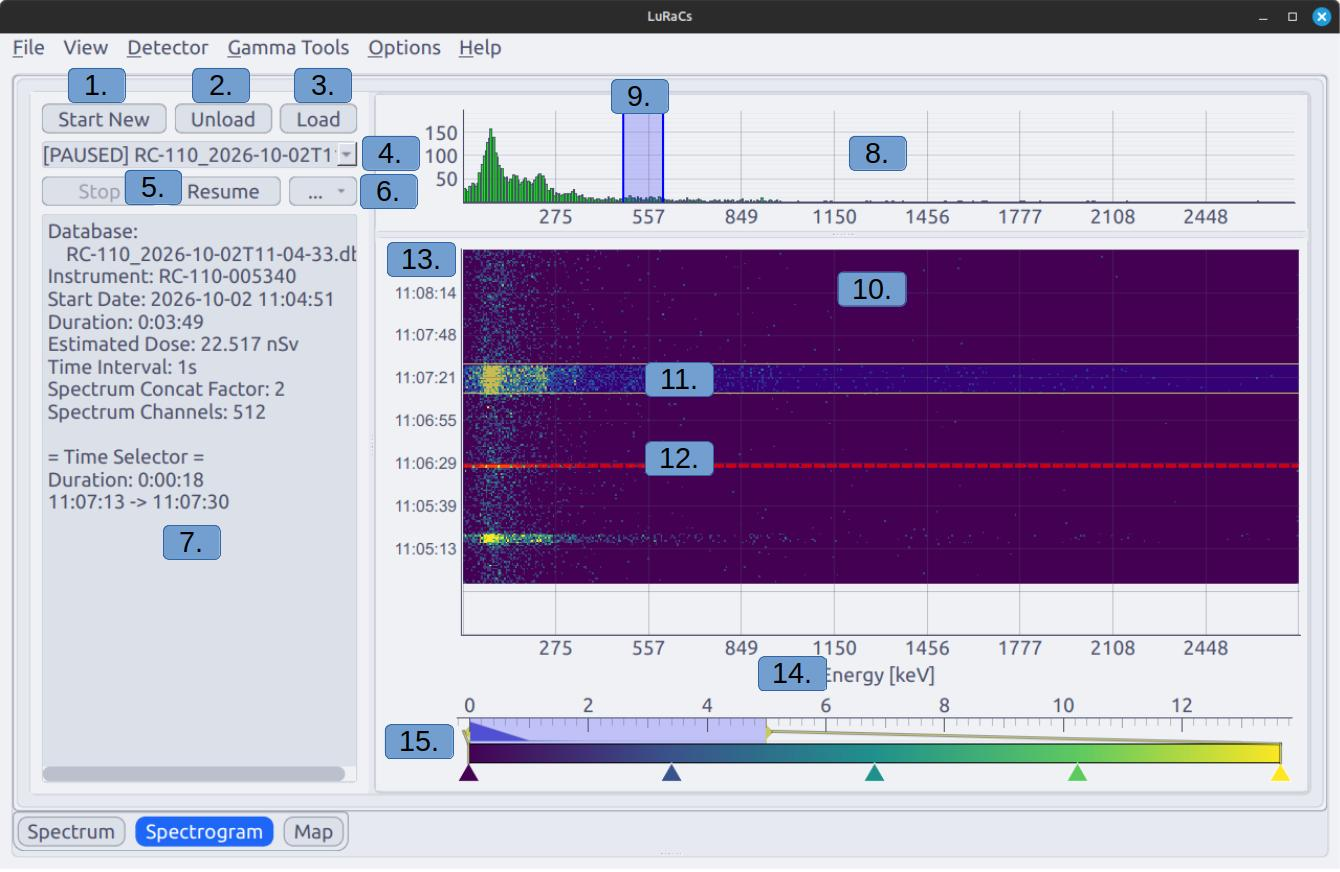
\includegraphics[width = .9\linewidth]{images/interface/spectrogram_view.jpg}
    \caption{Acquisition of a spectrogram with the \textit{Time Selector} active and one ROI.}
    \label{fig:spectrogram_view}

    \begin{flushleft}
        \begin{enumerate}
            \item Opens a dialog for starting a new spectrogram.
            \item Close the viewed spectrogram.
            \item Shortcut to the Data Library Spectrogram page, see section \ref{sec:data_store}.
            \item Toggle the currently loaded spectrograms. Status is shown to the left as [ACTIVE], [LOADED] or [PAUSED].
            \item Pause or Resume data collection, requires that the same detector used to collect the previous data is connected.
            \item Options menu, see \autoref{fig:spectrogram_options}
            \item Current information stored in the spectrogram and information about the \textit{Time Selector}, if active.
            \item Count histogram. Shows either total accumulated spectrum when loading a previously acquired spectrogram, summed channel counts inside the \textit{Time Selector}, if active, or counts in the latest row.
            \item ROI illustrated in the histogram, can be removed with Mouse-2.
            \item Waterfall diagram of the spectrogram.
            \item \textit{Time Selector} to study the summed spectra within a specific time interval. Can be toggled in the options menu (6.).
            \item Data break line, illustrates that the time between measured points exceeds the Time Interval. Can indicate a lost connection and thus caution should be taken to verify data integrity. Can be toggled in the options menu (6.).
            \item Y-axis displays the timestamps of when each row was measured.
            \item X-axis display spectrum energy, if calibrated.
            \item Color slider for the waterfall diagram. The color map can be changed by clicking Mouse-2 on the gradient bar.
        \end{enumerate}
    \end{flushleft}
\end{figure}

The spectrogram format is based around an SQLite database, see section \ref{sec:file_spectrogram} for further details on the format. The following data is stored for each time point in the spectrogram:

\begin{itemize}
    \item Timestamp.
    \item Average count rate measured since the last time point.
    \item Average dose rate measured since the last time point.
    \item Device temperature at the time the data is stored.
    \item Longitude at the time the data is stored, if a GPS is available.
    \item Latitude at the time the data is stored, if a GPS is available.
    \item Spectrum difference since the previous data point was stored, as compressed binary.
    \item Meta data, stored as a utf-8 encoded and zlib compressed json-string. Examples of stored metadata include extended GPS data.
\end{itemize}

\paragraph{Exporting a spectrogram} is done trough the Data Library, accessed via the \textit{Load}-button (2.).

\begin{figure}[H]
    \centering
    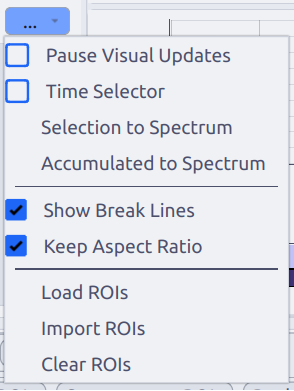
\includegraphics[width = .4\linewidth]{images/interface/spectrogram_options.png}
    \caption{Dropdown options menu in spectrogram pane, see \autoref{tab:spectrogram_options}.}
    \label{fig:spectrogram_options}
\end{figure}

\begin{table}[H]
    \centering
    \caption{Description of the possible operations in the spectrogram options menu}
    \label{tab:spectrogram_options}
    \begin{tabular}{p{.3\textwidth}p{.64\textwidth}}
    \toprule
    \textbf{Field} & \textbf{Description} \\ \midrule
    Pause Visual Updates & Stop the view spectrogram from updating while the measurement is still on going in the background. \textbf{This does not stop the recording of the spectrogram}. \\
    Time Selector & Add a selected ROI in the spectrogram (11.) that can indicate the specific time interval, as opposed to all other ROIs that have energy bounds, and show the sum over time of the channels in the top count histogram (8.). \\
    Selection to Spectrum & Export the data within a selected time interval to the Data Library as a spectrum. \\
    Accumulated to Spectrum & Export the accumulated counts to the Data Library as a spectrum. \\
    Show Break Lines & If the red lines (12.) indicating if the interval between two rows exceed the specified save interval should be shown. \\
    Keep Aspect Ratio & If the pixels in the spectrogram should always be square. For detectors with many channels it can be useful to turn this off. If this option is off the pixels in the spectrogram may not align with the corresponding bar in the count histogram. \\
    Load ROIs & Shortcut to the ROI tab of the Data Library. \\
    Import ROIs & Load ROIs from a LuRaCs XML-file. \\
    Clear ROIs & Remove all spectrogram ROIs \\
    \bottomrule
    \end{tabular}
\end{table}